%% =============================================================================
%% LOCAL DEPLOYMENT
%% =============================================================================

\section{Fully local deployment} \label{sec:local}

While cloud-hosted language models offer convenience and capability, many
use cases require complete data isolation: proprietary business data,
personally identifiable information under privacy regulations, or
air-gapped environments. This section describes the fully local deployment
configuration, where all components---including the language model---run
on the user's machine.

\subsection{Architecture}

Figure~\ref{fig:local-architecture} illustrates the local deployment
architecture. The key difference from cloud deployment is that the LLM
runs locally via Ollama \citep{Ollama}, eliminating all external network
communication. User queries, tool calls, and results never leave the
local machine.

\begin{figure}[htbp]
\centering
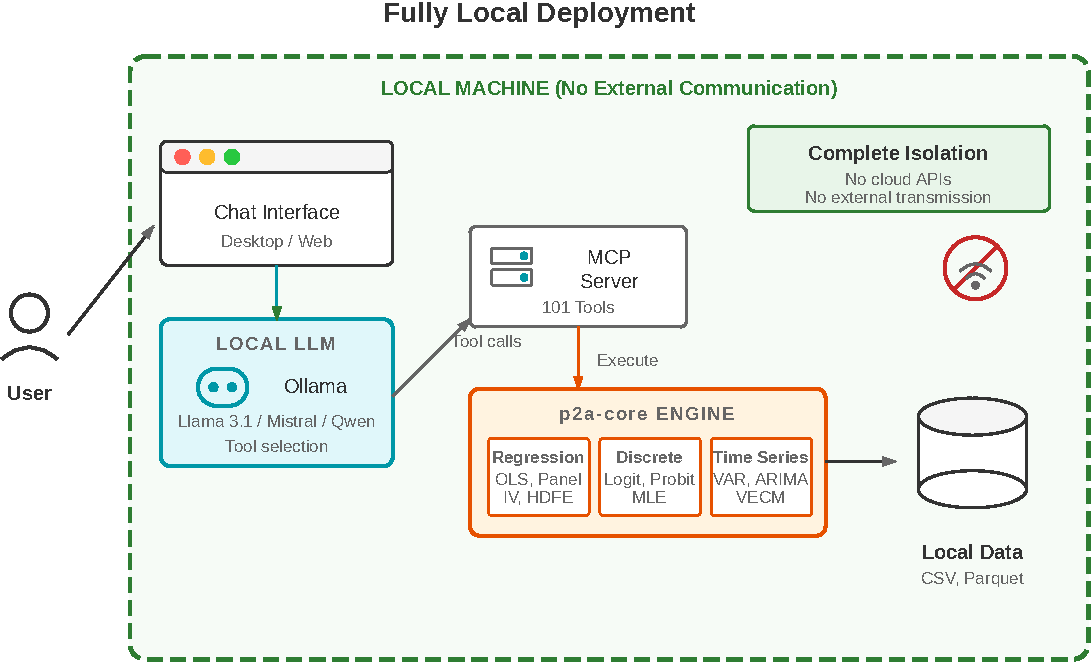
\includegraphics[width=0.9\textwidth]{figures/local_architecture}
\caption{Fully local deployment architecture. All components run on the
user's machine: Ollama hosts the language model, which communicates with
the MCP server to execute analytics methods in p2a-core. No data or
queries are transmitted externally.}
\label{fig:local-architecture}
\end{figure}

The local configuration requires:
\begin{itemize}
  \item Ollama runtime with a function-calling-capable model
  \item \pkg{prompt2analytics} MCP server
  \item Sufficient RAM for both the model and data processing
\end{itemize}

\subsection{Model selection for tool calling}

The chat-first architecture significantly reduces the capability
requirements for the local LLM. Rather than generating statistical code
from scratch---a task requiring deep understanding of matrix algebra,
numerical methods, and language-specific APIs---the model only needs to:
\begin{enumerate}
  \item Parse the user's natural language request
  \item Select appropriate tools from the MCP schema
  \item Generate correctly-formatted tool call parameters
  \item Interpret and explain the returned results
\end{enumerate}

This constrained task enables smaller, more efficient models to perform
effectively. The Berkeley Function Calling Leaderboard (BFCL) provides
standardized evaluation of function calling capabilities across models
\citep{BFCL:2024}. Recent research demonstrates that fine-tuned small
language models can match or exceed larger models on targeted tool
selection tasks \citep{Patil+Zhang+Song+Gonzalez:2023}.

% TODO: Add specific model recommendations and benchmarks
% Candidates: Llama 3.1 8B, Mistral 7B, Qwen 2.5, fine-tuned specialists

Based on preliminary evaluation, the following models provide reliable
tool selection for econometric methods:

\paragraph{Recommended models.}
\begin{description}
  \item[Llama 3.1 8B-Instruct] Best overall balance of capability and
    resource requirements. Requires 8GB+ RAM.
  \item[Mistral 7B-Instruct] Lower resource requirements with strong
    function calling performance.
  \item[Qwen 2.5 7B] Competitive tool-use performance, particularly for
    structured parameter generation.
\end{description}

Larger models (70B+) provide improved reasoning for complex analytical
decisions but require substantial hardware (64GB+ RAM or GPU offloading).

\subsection{Evaluation methodology}

Evaluating local LLM performance for econometric tool selection requires
assessing multiple dimensions:

\paragraph{Tool selection accuracy.}
Given a natural language description of an analytical task, does the
model select the appropriate statistical method? For example, a request
to ``estimate the causal effect of a policy change using pre/post data
with treatment and control groups'' should invoke difference-in-differences,
not standard OLS.

\paragraph{Parameter correctness.}
Does the model correctly populate tool parameters? This includes
identifying dependent and independent variables, specifying appropriate
options (robust standard errors, clustering variables), and handling
data type requirements.

\paragraph{Result interpretation.}
Can the model correctly interpret statistical output and communicate
findings to the user? This includes appropriate hedging about statistical
versus causal claims, identification of potential issues (multicollinearity,
weak instruments), and clear explanation of coefficient magnitudes.

% TODO: Add evaluation dataset and results
% Consider: synthetic benchmark, comparison across models, edge cases

\paragraph{Benchmark design.}
A comprehensive evaluation requires test cases spanning:
\begin{itemize}
  \item Method selection across all implemented categories (regression,
    panel, IV, discrete choice, time series)
  \item Ambiguous requests requiring model judgment
  \item Edge cases and error handling (missing variables, inappropriate
    method requests)
  \item Multi-step analytical workflows
\end{itemize}

Development of a standardized benchmark for econometric tool selection
remains an area for future work.

\subsection{Hardware requirements}

Table~\ref{tab:hardware} summarizes approximate hardware requirements
for local deployment configurations.

\begin{table}[htbp]
\centering
\caption{Hardware requirements for local deployment}
\label{tab:hardware}
\begin{tabular}{llll}
\toprule
Configuration & Model size & RAM & Notes \\
\midrule
Minimal & 7B & 16 GB & CPU inference, slower responses \\
Recommended & 8B & 32 GB & Comfortable headroom for data \\
Advanced & 70B & 64 GB+ & GPU recommended for reasonable speed \\
\bottomrule
\end{tabular}
\end{table}

The analytics engine itself has modest requirements; memory demands are
driven primarily by the language model and dataset size. Users with
limited hardware can offload model layers to disk at the cost of
inference speed.

\subsection{Privacy guarantees}

In the fully local configuration:
\begin{itemize}
  \item No network requests are made to external services
  \item All model inference occurs on local hardware
  \item Dataset contents never leave the machine
  \item Query history remains in local storage
\end{itemize}

This configuration is suitable for analysis of sensitive data where
regulatory or policy constraints prohibit cloud processing. Users should
verify their Ollama configuration does not enable telemetry or external
model downloads during analysis sessions.

